\documentclass[tikz,border=6pt]{standalone}
\usepackage{helvet}
\renewcommand{\familydefault}{\sfdefault}
\usetikzlibrary{arrows.meta,positioning}
\begin{document}
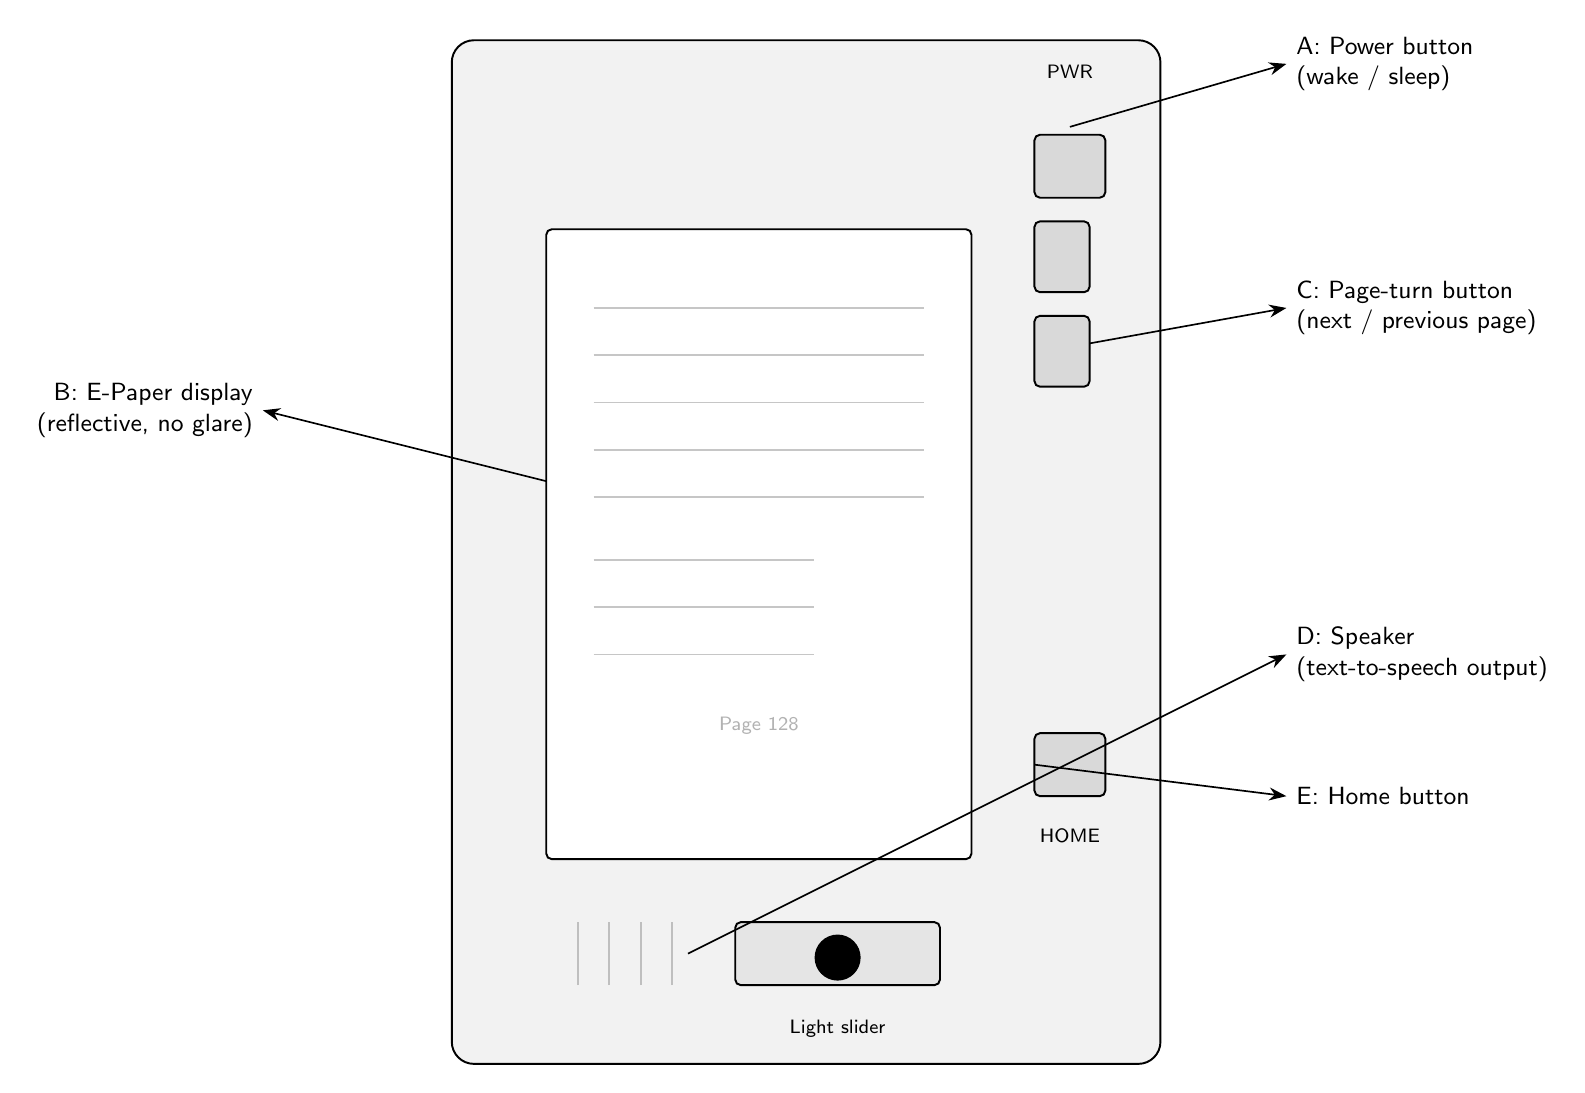
\begin{tikzpicture}[line width=0.7pt, font=\sffamily\small]

% ---- device body -----------------------------------------------------------
\draw[fill=gray!10, draw=black, rounded corners=8pt] (0,0) rectangle (9,13);

% ---- e-ink screen ----------------------------------------------------------
\draw[fill=white, draw=black, rounded corners=2pt] (1.2,2.6) rectangle (6.6,10.6);
% text lines on the page (thin strokes only)
\foreach \y in {9.6,9.0,8.4,7.8,7.2} { \draw[gray!45, line width=0.6pt] (1.8,\y) -- (6.0,\y); }
\foreach \y in {6.4,5.8,5.2}         { \draw[gray!45, line width=0.6pt] (1.8,\y) -- (4.6,\y); }
\node[gray!60, font=\sffamily\scriptsize] at (3.9,4.3) {Page 128};

% ---- controls --------------------------------------------------------------
% power button (top right)
\draw[fill=gray!30, rounded corners=2pt] (7.4,11.0) rectangle (8.3,11.8);
\node[font=\sffamily\scriptsize] at (7.85,12.6) {PWR};
% page-turn buttons (right column, between screen edge and body edge)
\draw[fill=gray!30, rounded corners=2pt] (7.4,8.6) rectangle (8.1,9.5);
\draw[fill=gray!30, rounded corners=2pt] (7.4,9.8) rectangle (8.1,10.7);
% home button
\draw[fill=gray!30, rounded corners=2pt] (7.4,3.4) rectangle (8.3,4.2);
\node[font=\sffamily\scriptsize] at (7.85,2.9) {HOME};
% speaker slots (bottom left)
\foreach \x in {1.6,2.0,2.4,2.8} { \draw[gray!50, line width=0.8pt] (\x,1.0) -- (\x,1.8); }
% display lighting slider (bottom centre)
\draw[fill=gray!20, rounded corners=2pt] (3.6,1.0) rectangle (6.2,1.8);
\draw[fill=black, rounded corners=1pt] (4.9,1.35) circle (0.28);
\node[font=\sffamily\scriptsize] at (4.9,0.45) {Light slider};

% ---- callouts --------------------------------------------------------------
% right-hand callouts (power, page-turn, home)
\draw[-{Stealth[length=2.2mm]}, line width=0.6pt] (7.85,11.9) -- (10.6,12.7)
  node[right, font=\sffamily\small, align=left] {A: Power button\\(wake / sleep)};
\draw[-{Stealth[length=2.2mm]}, line width=0.6pt] (8.1,9.15) -- (10.6,9.6)
  node[right, font=\sffamily\small, align=left] {C: Page-turn button\\(next / previous page)};
\draw[-{Stealth[length=2.2mm]}, line width=0.6pt] (7.4,3.8) -- (10.6,3.4)
  node[right, font=\sffamily\small, align=left] {E: Home button};
% speaker callout (rises from bottom-left, stays below the screen)
\draw[-{Stealth[length=2.2mm]}, line width=0.6pt] (3.0,1.4) -- (10.6,5.2)
  node[right, font=\sffamily\small, align=left] {D: Speaker\\(text-to-speech output)};
% screen callout from the LEFT edge of the device (keeps the right side clean)
\draw[-{Stealth[length=2.2mm]}, line width=0.6pt] (1.2,7.4) -- (-2.4,8.3)
  node[left, font=\sffamily\small, align=right] {B: E-Paper display\\(reflective, no glare)};

\end{tikzpicture}
\end{document}
